
\chapter{Einleitung}
\label{Einleitung}

Im Rahmen der Vorlesung Virtual Reality des Wintersemesters 18/19 wurden am Beispiel von Parameterkurven in der Ebene prototypisch dargestellt.
Parameterkurven haben Eigenschaften, die sich nur abstrakt auf Papier bzw. zweidimensional darstellen lassen.
In der UnityEngine besteht die Möglichkeit die Parameterkurven mittels Virtual Reality darzustellen.  
Diese Projektarbeit zeigt exemplarisch drei verschiedene Parameterkurven, um Eigenschaften der Kurven erlebbar zu machen. 
Die Idee lässt sich erweitern und könnte zukünfitg auch der Illustration von Dingen wie Ebenen im $R^{3}$ dienen.

\chapter{Verwendete Technologie}
\label{Technologie}
\section{Unity}
Unity ist eine Grafik-Engine, mit deren Hilfe 3D-Anwendungen realisiert werden. Es exisitert ein integrierter Editor, der ähnlich einem 3D-Grafik Programm, dazu verwendet wird die entsprechende Umgebung zu gestalten. Die fertige Anwendung bzw. das Spiel können für unterschiedlichste Plattformen von Android bis hin zu Linux erzeugt werden. Diese Anwedungen sind unabhängig von der Unity Entwicklungsumgebung lauffähig. Es wird ein Kompilat mit Abhänigkeiten und Ressourcen erzeugt.

\subsection{SciptEngine}
Unity stellt eine ScripEngine zur Verfügung, mit deren Hilfe derer die Umgebung und die darin vorhandenen Objekte beinflusst werden kann. Als Sprache für die Skripte kommt C\# zum Einsatz. Die Logik und der Ablauf der Ereignisse in der Anwendung werden durch Skripte festgelegt. Als Framework kommt das \emph{Mono Framework} zum Einsatz, eine Open Source Implementierung von Microsofts \emph{.NET Framework}.

\subsection{Prefabs}

\begin{figure}[h!]
	\centering
	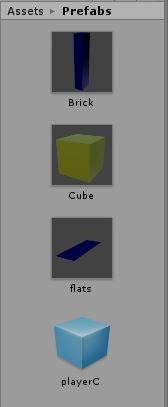
\includegraphics[scale=1]{bilder/prefabs.jpg}
	\caption{Im Projekt verwendete Prefabs}
\end{figure}

Prefabs - PreFabricates, sind bereits vorgefertigte Objekte, die Instanziiert werden müssen. Dies kann auf verschiedenen Wegen geschehen, in diesem Projekt wurden die Prefabs im Unity Editor erzeugt und per Script instantiiert.


\subsection{SteamVR Plugin für Unity}
Es existiert ein Plugin für die HTC Vive, eine VR-Brille. Dieses Plugin ist über den in Unity integrierten Asset Store zu beziehen. Es beinhaltet unter anderem sogenannte Prefabs, vorgefertigte Objekte, die in eine Szene eingesetzt werden können. Damit die Vive inklusive ihrer Controller funktioniert müssen die Prefabs [Steam VR] und [Camera Rig] in die Szene eingesetzt werden. 

\section{JetBrains Rider}
\label{Rider}
Die Standart Entwicklungsumgebung für Unity ist \emph{Microsoft Visual Studio 2017 in der Community Edition (kostenlos)}. Grundsätzlich ist jede IDE die C\# unterstüzt geeignet. Visual Studio 2017 und JetBrains Rider bieten zudem die Möglichkeit, sich an den Unity Prozess anzuhängen und einen Debugger einzusetzen. 

In diesem Projekt wurde Rider verwendet, da im Schwerpunkt auf Computern mit den Betriebssystem MacOS X entwickelt wurde und die Rider IDE in dieser Umgebung performanter und agiler ist.


\section{HTC Vive}
\label{Vive}
Das Zielmedium der Anwendung ist die HTC Vive, eine VR-Brille. Die Konfiguration an der Hochschule beinhaltet eine Brille, zwei Controller (einer Pro Hand) und die Sensoren, um die Position und Ausrichtung des Spielers im Raum zu erfassen. 
Der eingesetzte PC ist ein potenter Spielecomputer mit entsprechender Grafikhardware.

 